\begin{activity} \label{A:7.3.1}  
Consider the differential equation:
$$
  \frac{dy}{dt} = 6y-y^2
$$
\ba
\item Sketch the slope field for this differential equation on the axes below.

\begin{center}
  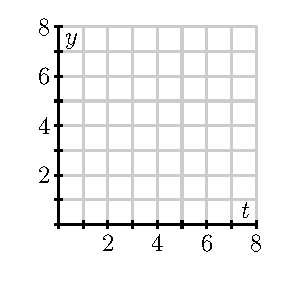
\includegraphics{figures/7_3_slopefield.eps}
\end{center}

\item Identify any equilibrium solutions and determine whether they
  are stable or unstable.   

\item What is the long-term behavior of the solution that satisfies the initial
  value $y(0) = 1$?

\item Using the initial value $y(0) = 1$, use Euler's method with
  $\Delta t = 0.2$ to approximate the solution at $t_i = 0.2, 0.4,
  0.6, 0.8$, and $1.0$.  Sketch the points $(t_i, y_i)$ on the axes provided.

\medskip
\begin{minipage}[t]{4in}
  \begin{tabular}{|c|c|c|c|c|}
  \hline
  $t_i$&$y_i$&$dy/dt$&$\Delta y$\\
  \hline
  \hline
  \vphantom{\Huge{M}}0.0&1.0000&\hphantom{1.0000}&\hphantom{0.2000} \\
  \hline
  \vphantom{\Huge{M}}0.2&\hphantom{MMMMMM} 
  & \hphantom{MMMMMM} & \hphantom{MMMMMM} \\
  \hline
  \vphantom{\Huge{M}}0.4& & & \\
  \hline
  \vphantom{\Huge{M}}0.6& & & \\
  \hline
  \vphantom{\Huge{M}}0.8& & & \\
  \hline
  \vphantom{\Huge{M}}1.0& & & \\
  \hline
\end{tabular}
\end{minipage}
\begin{minipage}[c]{2in}
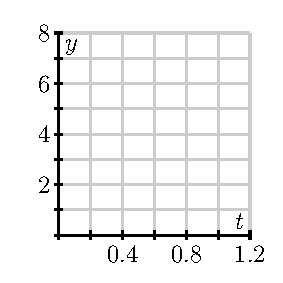
\includegraphics{figures/7_3_euler_empty_2.eps}
\end{minipage}

\item What happens if we apply Euler's method to approximate the
  solution with $y(0) = 6$?

\ea
\end{activity}
\begin{smallhint}
\ba
	\item Small hints for each of the prompts above.
\ea
\end{smallhint}
\begin{bighint}
\ba
	\item Big hints for each of the prompts above.
\ea
\end{bighint}
\begin{activitySolution}
\ba
	\item Solutions for each of the prompts above.
\ea
\end{activitySolution}
\aftera